% Figura 3: arquitectura basica de una GAN
% Compilar: pdflatex fig03_gan.tex
%           pdftoppm -png -r 300 -singlefile fig03_gan.pdf ../output/thesis_figures/fig03_gan
\documentclass[border=8pt]{standalone}
\usepackage[utf8]{inputenc}
\usepackage[T1]{fontenc}
\usepackage{tikz}
\usetikzlibrary{positioning,arrows.meta,calc}

\begin{document}
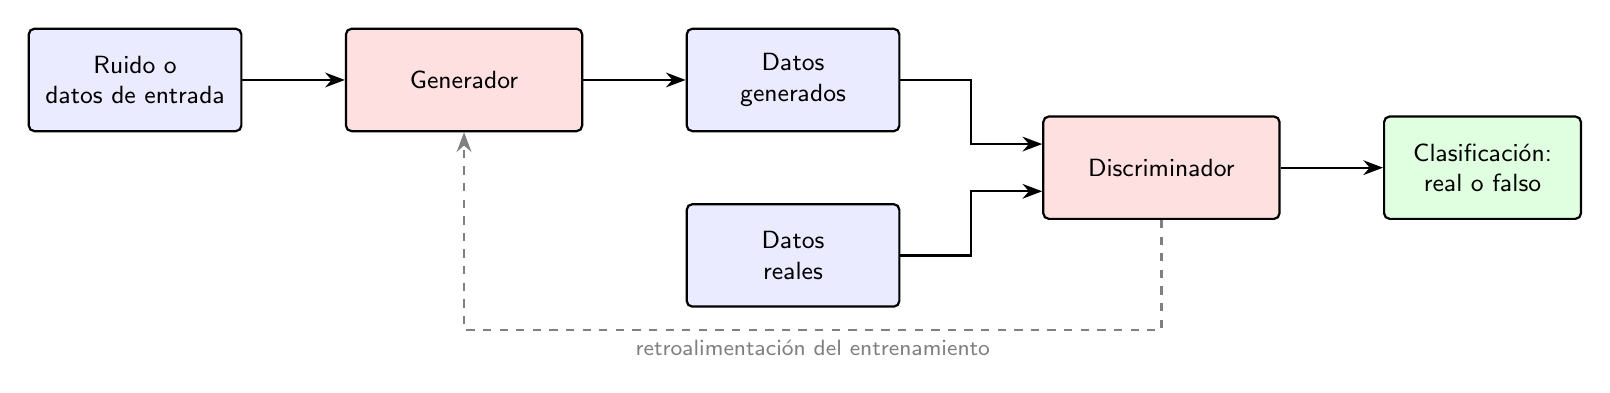
\begin{tikzpicture}[
    font=\sffamily\small,
    node distance=9mm and 13mm,
    dato/.style={draw, rounded corners=2pt, fill=blue!8, minimum width=27mm,
                 minimum height=13mm, align=center, thick},
    red/.style={draw, rounded corners=2pt, fill=red!12, minimum width=30mm,
                minimum height=13mm, align=center, thick},
    salida/.style={draw, rounded corners=2pt, fill=green!12, minimum width=25mm,
                   minimum height=13mm, align=center, thick},
    flecha/.style={-{Stealth[length=2.5mm]}, thick},
    retro/.style={-{Stealth[length=2.5mm]}, thick, dashed, gray}
]

\node[dato]                                  (entrada) {Ruido o\\datos de entrada};
\node[red,    right=of entrada]              (gen)     {Generador};
\node[dato,   right=of gen]                  (falsos)  {Datos\\generados};
\node[dato,   below=of falsos]               (reales)  {Datos\\reales};
\node[red,    right=18mm of $(falsos.east)!0.5!(reales.east)$] (disc) {Discriminador};
\node[salida, right=of disc]                 (verdad)  {Clasificaci\'on:\\real o falso};

\draw[flecha] (entrada) -- (gen);
\draw[flecha] (gen) -- (falsos);
\draw[flecha] (falsos.east) -- ++(9mm,0) |- ([yshift=3mm]disc.west);
\draw[flecha] (reales.east) -- ++(9mm,0) |- ([yshift=-3mm]disc.west);
\draw[flecha] (disc) -- (verdad);

\draw[retro] (disc.south) -- ++(0,-14mm) -| (gen.south)
    node[pos=0.25, below, font=\sffamily\footnotesize, text=gray]
    {retroalimentaci\'on del entrenamiento};

\end{tikzpicture}
\end{document}
